\documentclass{article}
\usepackage[utf8]{inputenc}
\usepackage{hyperref}
\usepackage{amsmath}
\usepackage{tikz}
\usepackage{adjustbox}


\title{Exposé: How can LLMs be effectively used for the classification and transfer between language levels in German?}
\author{Elias-Leander Ahlers}
\date{\today}

\begin{document}

\maketitle

\section{Introduction}

Large Language Models (LLMs) have gained significant attention in recent years due to their
impressive performance in various natural language processing tasks. Models, such as GPT-3,
Gemini and LLaMA, have demonstrated the ability to generate human-like text, translate languages, and
perform a wide range of other language-related tasks. My thesis will investigate the capabilities
of LLMs in the classification and transfer of texts across different proficiency levels of the
German language as outlined by the Common European Framework of Reference for Languages (CEFR).
The CEFR categorizes language proficiency into six distinct levels ranging from A1 (beginner) to
C2 (proficient), providing a clear framework for evaluating an individual's language skills.

\textit{Firstly}, the thesis will address the classification challenge, where an LLM is tasked with 
determining the CEFR level of a given text. This involves processing and understanding texts in
German to accurately assign them to the correct language proficiency category. 

\textit{Secondly}, the project will explore the model's capability for language transfer: Modifying
a text to conform to a specific CEFR level as designated by the user while maintaining the original
content and meaning. This feature aims to modify the text in a way that aligns with the target
proficiency, making the technology very useful for customized language learning and evaluation.

The relevance of the topic to computer science comes from the suitability of LLMs for this type of
text processing. The Transformer architecture currently used in most LLMs was originally developed 
to allow translations between different languages \cite{attention_is_all_you_need}. Applying this technology to the transfer between
language levels is the next logical step. The project is also relevant to the field of language 
education, as it can provide valuable tools for teachers and learners to assess and improve language
skills. It can be used to automatically classify texts according to their language level, as well as
to adjust texts to match a specific language level.

\section{Related Work}
The landscape of existing research in the area of text classification by language proficiency levels 
already has some studies that employ specialized models (e.g . SVMs instead of LLMs) \cite{automated_assessment} 
\cite{german_simplification} \cite{proficiency_classification}. These models are typically
solutions designed to categorize texts based on established language proficiency frameworks such as
the CEFR. While effective in their capacity as classifiers, these models are not based on the broader,
more flexible architectures of LLMs and can not be used for the transfer task.

Also, the field of research utilizing LLMs for language proficiency tasks has been primarily
focused on English. This presents a significant gap in the literature, as the unique structures
of different languages play a crucial role in the performance of these models as they are depended on
their training data. This is particularly relevant for the German language, where the linguistic
patterns and structures differ significantly from English.

Moreover, initial explorations into the capabilities of LLMs in handling German texts have shown
mixed outcomes. While existing foundation models generally perform decently in classifying texts
into correct CEFR levels, they do significantly worse when tasked with adapting text to match a
specific language proficiency level, particularly when transferring to complex levels (B2+) (Where
grammar becomes more complex and important). Observations indicate that these models, many of which
are pre-trained mainly on English data, tend to default towards English grammar patterns when
attempting language level transfer. This is another area where the research is lacking, and my
thesis aims to address this gap regarding the German language.

\section{Research Question}
\begin{quote}
"How can LLMs be effectively used for the classification and transfer between language levels in German?"
\end{quote}

\section{Methodology}
The research methodology focuses on the use of LLMs. Initially, the possibility of adapting existing 
approaches to the current problem will be explored, particularly transferring parts of techniques 
from English to German research. But as they are not directly transferable, due to not using LLMs
and the differences in language structure, the main focus will be on the development of new methods.

\subsection{Using existing model and attempting prompting}
The first approach involves using an existing LLM, possibly a German fine tuned LLaMA model \cite{llama_german_finetune}, and 
experimenting with targeted prompting to classify and transfer texts between language levels.
This will involve developing prompts that guide the model towards recognizing and maintaining the
language levels. Possible strategies include providing examples in the prompt for different levels,
adjusting the prompt structure, and experimenting with different parameters to achieve the desired
results. This approach aims to leverage the existing capabilities of the model while adapting it to
the specific requirements of the task. Due to some tests already showing good results, this approach
seem promising regarding the classification task, but the transfer task is still challenging.
Therefore the second approach is also considered:

\subsection{Fine-tuning an LLM}
The second approach involves fine-tuning an existing LLM with appropriate training data to better
align the model with recognizing and maintaining language levels. This method requires a significant
amount of high quality training data that is labeled with the respective CEFR levels. The model will
be fine-tuned on this data to learn the patterns and structures of texts at different German language
levels. The goal is to improve the model's performance in classifying and transferring texts between
language levels. Bur the focus will be on the transfer task, as the classification task is already
promising with the first approach and should transfer to the fine-tuned model as well. The major
challenge here is to gather a large enough dataset with high quality labels and data, as this is
crucial for the success of the fine-tuning process.

\subsection{Benchmarking}
For both methods I need a way to evaluate the approaches. Therefore, I plan to develop a benchmark
that can be used to assess the effectiveness of the models. This benchmark will consist of two parts
that correspond to the classification and transfer tasks. The first part is a simple test where the
model has to classify texts into the correct CEFR levels. The second part is more complex and 
involves transferring texts between different language levels while maintaining the original content
and meaning. This is harder to evaluate, as it isn't a simple classification task that can be
automatically validated. Therefore, manual evaluation or another LLM will be needed. But that is 
still to be determined and will be part of the research/thesis.

\section{Expected Results}
I anticipate - based on the initial tests - that the classification of language proficiency levels by CEFR can 
be achieved more or less reliably through prompting. The default behavior of the models is already
very promising in this regard. And with further techniques and adjustments like few-shot prompting
and other strategies, the classification task should be solvable. 

The transfer task is more challenging and will likely require fine-tuning the model. The model
will need to be trained on a large dataset with high quality labels to learn the patterns and
structures of texts at different language levels. But with the right data and training, the model
should be able to transfer texts between language levels while maintaining the original content
and meaning.

Relevant metrics, in this case a benchmark, are also essential for evaluating the effectiveness of
the models. But I also expect that this is solvable and can be developed as part of the research.
The first part is rather simple, as it is a classification task that can be automatically validated.
The second part is more difficult and requires complex evaluation.


\section{Schedule}
% \begin{itemize}
%     \item 3 weeks: Literature review and research on existing models and approaches
%         + Collecting data (parts of it are required for the benchmark)
%     \item 2 weeks: Development of the benchmark for evaluation
%     \item 2 weeks: Experimenting with prompting techniques for existing LLMs
%     \item 2 weeks: Preparation for fine-tuning
%     \item 4 weeks: Fine-tuning the LLM and training on the dataset
%     \item 2 weeks: Evaluation of the models and comparison of results
%     \item 4 weeks: Writing the thesis and preparing the final presentation
%     \item 2 weeks: Buffer for unexpected delays
% \end{itemize}

\begin{adjustbox}{width=\textwidth}
    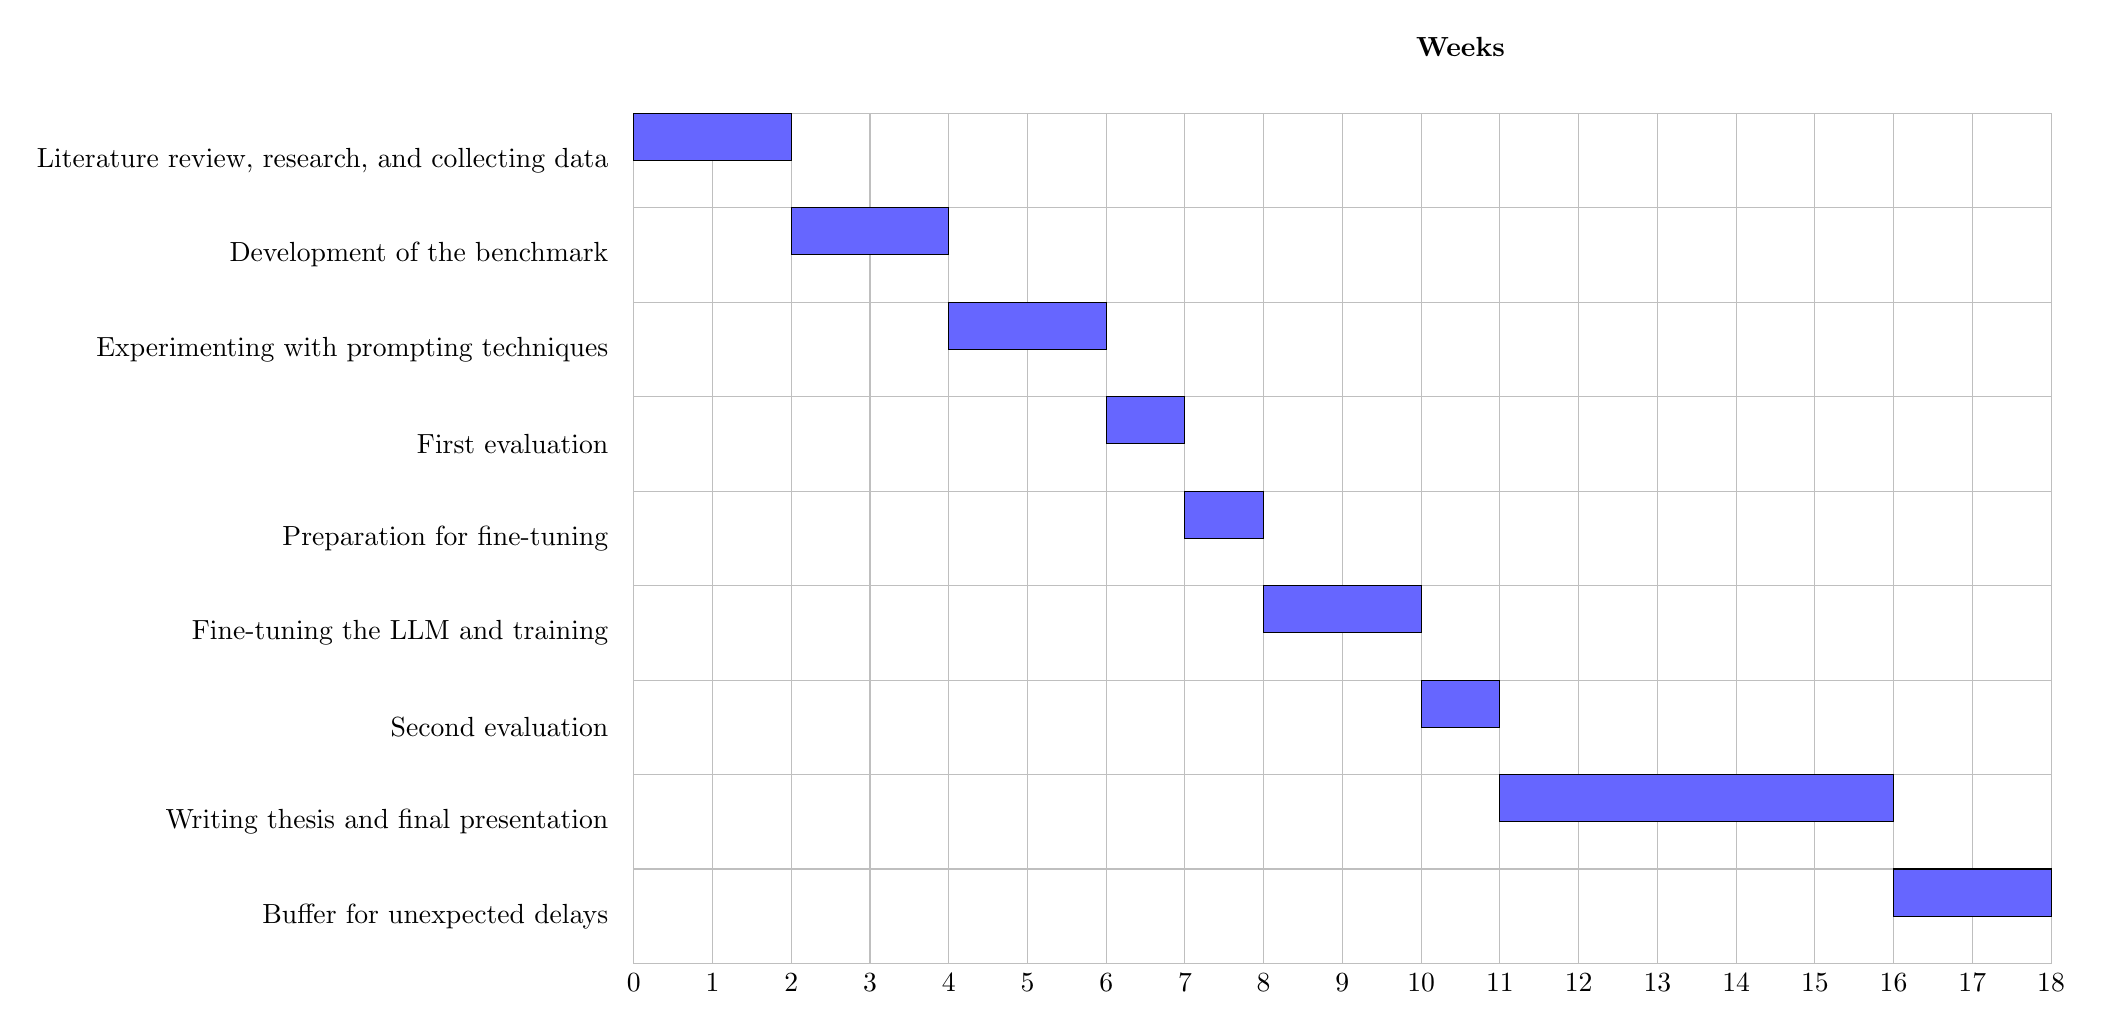
\begin{tikzpicture}[x=1.0cm, y=1.2cm]

    \newcommand{\scheduleWidth}{18}
    \newcommand{\scheduleHeight}{9}
    
    \foreach \y in {0,1,...,\scheduleHeight} {
        \draw[gray!50] (0,\y) -- (\scheduleWidth,\y);
    }
    
    \foreach \x in {0,1,...,\scheduleWidth} {
        \draw[gray!50] (\x,0) -- (\x,\scheduleHeight);
    }
    
    \node[anchor=east] at (-0.2, 8.5) {Literature review, research, and collecting data};
    \node[anchor=east] at (-0.2, 7.5) {Development of the benchmark};
    \node[anchor=east] at (-0.2, 6.5) {Experimenting with prompting techniques};
    \node[anchor=east] at (-0.2, 5.5) {First evaluation};
    \node[anchor=east] at (-0.2, 4.5) {Preparation for fine-tuning};
    \node[anchor=east] at (-0.2, 3.5) {Fine-tuning the LLM and training};
    \node[anchor=east] at (-0.2, 2.5) {Second evaluation};
    \node[anchor=east] at (-0.2, 1.5) {Writing thesis and final presentation};
    \node[anchor=east] at (-0.2, 0.5) {Buffer for unexpected delays};
    
    \draw[fill=blue!60] (0, 8.5) rectangle (2, 9); % Literature review
    \draw[fill=blue!60] (2, 7.5) rectangle (4, 8); % Development of the benchmark
    \draw[fill=blue!60] (4, 6.5) rectangle (6, 7); % Experimenting with prompting techniques
    \draw[fill=blue!60] (6, 5.5) rectangle (7, 6); % First evaluation
    \draw[fill=blue!60] (7, 4.5) rectangle (8, 5); % Preparation for fine-tuning
    \draw[fill=blue!60] (8, 3.5) rectangle (10, 4); % Fine-tuning the LLM and training
    \draw[fill=blue!60] (10, 2.5) rectangle (11, 3); % Second evaluation
    \draw[fill=blue!60] (11, 1.5) rectangle (16, 2); % Writing thesis and final presentation
    \draw[fill=blue!60] (16, 0.5) rectangle (18, 1); % Buffer for unexpected delays
    
    \foreach \x in {0,...,\scheduleWidth} {
        \node[anchor=north] at (\x, 0) {\x};
    }
    
    \node[anchor=south] at (10.5, 9.5) {\textbf{Weeks}};
    
    \end{tikzpicture}
\end{adjustbox}

\section{Conclusion}
In this exposé I explored the application of LLMs in classifying and adapting German text to
different proficiency levels as per the CEFR. The research aims to investigate the effectiveness
of LLMs in these tasks and develop new methods to improve their performance in two distinct areas:
classification and language level transfer. The project will involve experimenting with existing
models using prompting techniques and fine-tuning an LLM to archive the desired results - Mainly
archiving the transfer task. The research will also include the development of a benchmark to
evaluate the models' performance quantitatively and aid in the comparison of different approaches
and their effectiveness.

\newpage


\begin{thebibliography}{unsrt}
    \bibitem{attention_is_all_you_need}
    Vaswani, Ashish, et al. "Attention is all you need." Advances in neural information processing systems 30 (2017).
    \bibitem{automated_assessment}
    Szügyi, Edit, et al. "Automated Assessment of Language Proficiency on German Data." KONVENS. 2019.
    \bibitem{german_simplification}
    Spring, Nicolas, Annette Rios, and Sarah Ebling. "Exploring German multi-level text simplification." (2021): 1339-1349.
    \bibitem{proficiency_classification}
    Hnatkowska, Bogumila, and Damian Wawrzyniak. "Proficiency level classification of foreign language learners using machine learning algorithms and multilingual models." International Conference on Computational Collective Intelligence. Cham: Springer International Publishing, 2022.
    \bibitem{llama_german_finetune}
    Freely available LLaMA 2 German fine-tune by Jan Philipp Harries \url{https://github.com/jphme/EM_German}
\end{thebibliography}

\end{document}
